\section*{Ejercicios de tipo test}
\addcontentsline{toc}{section}{Ejercicios de tipo test}



\begin{ejercicio}
Considera el siguiente código Python:

\begin{python}
datos = ["Lunes", "Martes", "Miércoles", "Jueves", "Viernes"]

archivo = open("dias.txt", "w")
for dia in datos:
    archivo.write(dia + "\n")
archivo.close()

archivo = open("dias.txt", "r")
contenido = archivo.read()
archivo.close()

print(contenido)
\end{python}

Después de ejecutar el código, ¿qué contendrá la variable \texttt{contenido}?

\begin{choices}
    \choice \texttt{"Lunes\textbackslash nMartes\textbackslash nMiércoles\textbackslash nJueves\textbackslash nViernes\textbackslash n"}
    \choice \texttt{"Lunes, Martes, Miércoles, Jueves, Viernes"}
    \choice \texttt{"Viernes, Jueves, Miércoles, Martes, Lunes"}
    \choice \texttt{"dias.txt"}
\end{choices}

\end{ejercicio}

\begin{ejercicio}
Considera el siguiente código Python:

\begin{python}
def contar_palabras(archivo_nombre):
    archivo = open(archivo_nombre, "r")
    contenido = archivo.read()
    archivo.close()
    palabras = contenido.split()
    return len(palabras)

archivo_texto = "texto.txt"

cantidad_palabras = contar_palabras(archivo_texto)

print("El archivo {} contiene {} palabras.".format(archivo_texto, cantidad_palabras))
\end{python}

Si el archivo \texttt{texto.txt} contiene el siguiente texto:\\

\begin{Verbatim}[frame=single]
La programación es divertida y útil. Python es un lenguaje de programación popular.
\end{Verbatim}

¿Cuántas palabras contiene el archivo?

\begin{choices}
    \choice 10
    \choice 12
    \choice 14
    \choice 16
\end{choices}

\end{ejercicio}

\begin{ejercicio}
Considera el siguiente código Python:

\begin{python}
def buscar_palabra(archivo_nombre, palabra_buscar):
    archivo = open(archivo_nombre, "r")
    contenido = archivo.read()
    archivo.close()
    palabras = contenido.split()
    return palabra_buscar in palabras

archivo_texto = "texto.txt"
palabra_a_buscar = "divertida"

encontrada = buscar_palabra(archivo_texto, palabra_a_buscar)

if encontrada:
    print("La palabra '{}' se encuentra en el archivo.".format(palabra_a_buscar))
else:
    print("La palabra '{}' no se encuentra en el archivo.".format(palabra_a_buscar))
\end{python}

Si el archivo \texttt{texto.txt} contiene el siguiente texto:\\

\begin{Verbatim}[frame=single]
La programación es divertida y útil. Python es un lenguaje de programación popular.
\end{Verbatim}

¿Qué mensaje se imprimirá al ejecutar el código?

\begin{choices}
    \choice "La palabra 'divertida' se encuentra en el archivo."
    \choice "La palabra 'útil' se encuentra en el archivo."
    \choice "La palabra 'divertida' no se encuentra en el archivo."
    \choice "La palabra 'útil' no se encuentra en el archivo."
\end{choices}

\end{ejercicio}

\begin{ejercicio}
Considera el siguiente código Python:

\begin{python}
archivo = open("datos.txt", "r")
contenido = archivo.read()
archivo.close()

print(contenido)
\end{python}

Si el archivo \texttt{datos.txt} contiene lo siguiente:\\

\begin{Verbatim}[frame=single]
Hola, Mundo!
Este es un archivo de prueba.
¡Espero que te diviertas programando en Python!
\end{Verbatim}

¿Cuál será la salida impresa por el código?

\begin{choices}
    \choice \texttt{"Hola, Mundo!\textbackslash nEste es un archivo de prueba.\textbackslash n¡Espero que te diviertas programando en Python!"}
    \choice \texttt{"Hola, Mundo!"}
    \choice \texttt{"Este es un archivo de prueba."}
    \choice \texttt{"¡Espero que te diviertas programando en Python!"}
\end{choices}

\end{ejercicio}

\begin{ejercicio}
Considera el siguiente código Python:

\begin{python}
datos = ["Manzana", "Banana", "Naranja", "Piña"]

archivo = open("frutas.txt", "w")
for fruta in datos:
    archivo.write(fruta + "\textbackslash n")
archivo.close()
\end{python}

¿Qué contendrá el archivo \texttt{frutas.txt} después de ejecutar el código?

\begin{choices}
    \choice \texttt{"Manzana\textbackslash nBanana\textbackslash nNaranja\textbackslash nPiña"}
    \choice \texttt{"ManzanaBananaNaranjaPiña"}
    \choice \texttt{"Piña\textbackslash nNaranja\textbackslash nBanana\textbackslash nManzana"}
    \choice \texttt{"frutas.txt"}
\end{choices}

\end{ejercicio}

\begin{ejercicio}
Considera el siguiente código Python:

\begin{python}
def contar_lineas(archivo_nombre):
    archivo = open(archivo_nombre, "r")
    lineas = archivo.readlines()
    archivo.close()
    return len(lineas)

archivo_entrada = "entrada.txt"
archivo_salida = "salida.txt"

lineas = contar_lineas(archivo_entrada)

archivo = open(archivo_salida, "w")
archivo.write(f"El archivo {archivo_entrada} tiene {lineas} líneas.")
archivo.close()
\end{python}

Si el archivo \texttt{entrada.txt} contiene 15 líneas de texto, ¿qué contendrá el archivo \texttt{salida.txt} después de ejecutar el código?

\begin{choices}
    \choice \texttt{"El archivo entrada.txt tiene 15 líneas."}
    \choice \texttt{"El archivo salida.txt tiene 15 líneas."}
    \choice \texttt{"El archivo entrada.txt tiene 150 líneas."}
    \choice \texttt{"El archivo salida.txt tiene 150 líneas."}
\end{choices}

\end{ejercicio}





\begin{ejercicio}
Considerar el siguiente programa: 


\begin{python}
f = open("hi.txt")
resultado = ""
for l in f:
    resultado += l[2]
print(resultado)
\end{python}

Y el siguiente fichero \verb+hi.txt+ en el mismo directoria que nuestro programa Python:
 
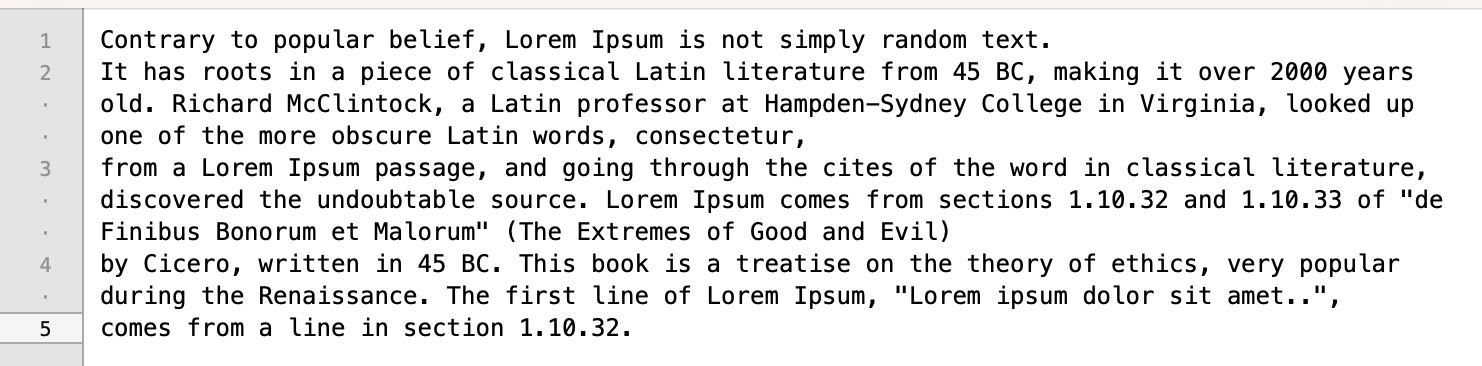
\includegraphics[width = 16cm]{book/Spanish/06_Ficheros/images/hi_ficherox.png}

\begin{choices}
    \choice \pythoninline{n o m} %CORRECT
    \choice \pythoninline{n deosn rm}
    \choice \pythoninline{ndeosnrm}
    \choice \pythoninline{TypeError: 'function' object f is not iterable}
\end{choices}

\end{ejercicio}

\begin{ejercicio}
    Considerar el siguiente programa:


\begin{python}
f = open("data.txt", "r")
c = int(f.read(1))
for i in range (1,5,2):
    line = f.readline().rstrip()
    if (line.find("a")):
        c = c+1
print(c)
f.close()
\end{python}
 
Y el siguiente fichero \texttt{data.txt} que se encuentra en el mismo directorio que el programa.
 
 \begin{python}
2023
¡Llegaron casi las vacaciones, yupi!
\end{python}

¿Qué sale?

\begin{choices}
      \choice \pythoninline{4} %CORRECT
    \choice  \pythoninline{ValueError: invalid literal for int() with base 10}
    \choice nada
  \choice \pythoninline{AttributeError: 'io.TextIOWrapper' object has no attribute 'readline'}
\end{choices}
\end{ejercicio}


